%%%%%%%%%%%%%%%%%%%%%%%%%%%%%%%%%%%%%%%%%
% Beamer Presentation
% LaTeX Template
% Version 1.0 (10/11/12)
%
% This template has been downloaded from:
% http://www.LaTeXTemplates.com
%
% License:
% CC BY-NC-SA 3.0 (http://creativecommons.org/licenses/by-nc-sa/3.0/)
%
%%%%%%%%%%%%%%%%%%%%%%%%%%%%%%%%%%%%%%%%%

%----------------------------------------------------------------------------------------
%	PACKAGES AND THEMES
%----------------------------------------------------------------------------------------

\documentclass{beamer}

\mode<presentation> {

% The Beamer class comes with a number of default slide themes
% which change the colors and layouts of slides. Below this is a list
% of all the themes, uncomment each in turn to see what they look like.

%\usetheme{default}
%\usetheme{AnnArbor}
%\usetheme{Antibes}
%\usetheme{Bergen}
%\usetheme{Berkeley}
%\usetheme{Berlin}
%\usetheme{Boadilla}
%\usetheme{CambridgeUS}
%\usetheme{Copenhagen}
%\usetheme{Darmstadt}
%\usetheme{Dresden}
%\usetheme{Frankfurt}
%\usetheme{Goettingen}
%\usetheme{Hannover}
%\usetheme{Ilmenau}
%\usetheme{JuanLesPins}
%\usetheme{Luebeck}
\usetheme{Madrid}
%\usetheme{Malmoe}
%\usetheme{Marburg}
%\usetheme{Montpellier}
%\usetheme{PaloAlto}
%\usetheme{Pittsburgh}
%\usetheme{Rochester}
%\usetheme{Singapore}
%\usetheme{Szeged}
%\usetheme{Warsaw}

% As well as themes, the Beamer class has a number of color themes
% for any slide theme. Uncomment each of these in turn to see how it
% changes the colors of your current slide theme.

%\usecolortheme{albatross}
%\usecolortheme{beaver}
%\usecolortheme{beetle}
%\usecolortheme{crane}
%\usecolortheme{dolphin}
%\usecolortheme{dove}
%\usecolortheme{fly}
%\usecolortheme{lily}
%\usecolortheme{orchid}
%\usecolortheme{rose}
%\usecolortheme{seagull}
%\usecolortheme{seahorse}
%\usecolortheme{whale}
%\usecolortheme{wolverine}

%\setbeamertemplate{footline} % To remove the footer line in all slides uncomment this line
%\setbeamertemplate{footline}[page number] % To replace the footer line in all slides with a simple slide count uncomment this line

%\setbeamertemplate{navigation symbols}{} % To remove the navigation symbols from the bottom of all slides uncomment this line
}
\usepackage{graphicx} % Allows including images
\usepackage{booktabs} % Allows the use of \toprule, \midrule and \bottomrule in tables

\usepackage{array}

\usepackage{algorithm,algorithmic}
\usepackage{multicol}
\usepackage{caption,subcaption}
\newcolumntype{V}[1]{>{\centering\arraybackslash} m{#1} }
\newcolumntype{L}[1]{>{\arraybackslash} m{#1} }

\pdfpageattr {/Group << /S /Transparency /I true /CS /DeviceRGB>>}%solves color issues brought by inserting pdf figures
%----------------------------------------------------------------------------------------
%	TITLE PAGE
%----------------------------------------------------------------------------------------

\title[Master Thesis Presentation]{An assistive handwashing system with emotional intelligence}
% The short title appears at the bottom of every slide, the full title is only on the title page

\author{Luyuan Lin} % Your name
\institute[UWaterloo] % Your institution as it will appear on the bottom of every slide, may be shorthand to save space
{
University of Waterloo \\ % Your institution for the title page
\medskip
\textit{Supervisor:
\newline Jesse Hoey
} % Your email address
}
\date{\today} % Date, can be changed to a custom date

\begin{document}

\begin{frame}
\titlepage % Print the title page as the first slide
\end{frame}

\begin{frame}
\frametitle{Overview} % Table of contents slide, comment this block out to remove it
\tableofcontents % Throughout your presentation, if you choose to use \section{} and \subsection{} commands, these will automatically be printed on this slide as an overview of your presentation
\end{frame}

%----------------------------------------------------------------------------------------
%	PRESENTATION SLIDES
%----------------------------------------------------------------------------------------

%-----------------------------------------------------------------
\section{Problem Statement} 
% Sections can be created in order to organize your presentation into discrete blocks
% all sections and subsections are automatically printed in the table of contents as an overview of the talk
%------------------------------------------------
\subsection{Motivation}
\begin{frame}
\frametitle{Problem Statement - Motivation}
The COACH system
\begin{itemize}
\item is an assistive system helping with an elder's daily activities
\item monitors a user washing his/her hands
\item detects when the user has lost track of what he/she is doing
\item displays a prerecorded assistive prompt when needed
\item works well for some persons, but not as well for others
\end{itemize}
\pause
\vspace{0.3cm}
Using Emotional Intelligence in Assitive Systems
\begin{itemize}
\pause \item recognization of affective states
\pause \item generation of affective signals
\pause \item study of human emotions
\pause \item computationally modelling affective HCIs
\end{itemize}
\end{frame}

%------------------------------------------------
\subsection{Objectives}
\begin{frame}
\frametitle{Problem Statement - Objectives}
To augment the COACH system with an emotional reasoning engine based on BayesACT so that the augmented system:\\
\begin{itemize}
\pause \item is designed in a portable and extensible way
\pause \item runs in real-time from the perspective of the user group
\pause \item provides at least a level of functional assistance of as high quality as the COACH
\pause \item is able to tune the prompts in some way according to the emotional state of a user
\end{itemize}
\vspace{0.3cm}
\pause Note: The last objective is ill-defined, as the question of how exactly tuning prompts to users will be most effective is not clear at this point.
\end{frame}

%-----------------------------------------------------------------
\section{Basic Concepts}
%------------------------------------------------
\subsection{Affect Control Theory (ACT)}
\begin{frame}
\frametitle{Concepts - ACT}
Affect Control Theory (ACT)
\begin{itemize}
\item represents emotions as vectors that represent evaluation ($E$), potency ($P$), and activity ($A$) respectively
\pause \item describes social events by an Actor-Behaviour-Object (ABO) grammar
\pause \item ``fundamentals'' of identities and behaviours; shared between people within a same culture
\pause \item ``transient impressions'': emotional feelings of people evoked by a specific event
\end{itemize}
\begin{block}{The ACT Principal}
Actors work to experience transient impressions that are consistent with their fundamental sentiments.
\end{block}
\end{frame}

%------------------------------------------------
\subsection{Partially Observable Markov Decision Process (POMDP)}
\begin{frame}
\frametitle{Concepts - POMDP}
Partially Observable Markov Decision Process (POMDP)
\vspace{.3cm}
\begin{columns}[c]
\column{.5\textwidth}
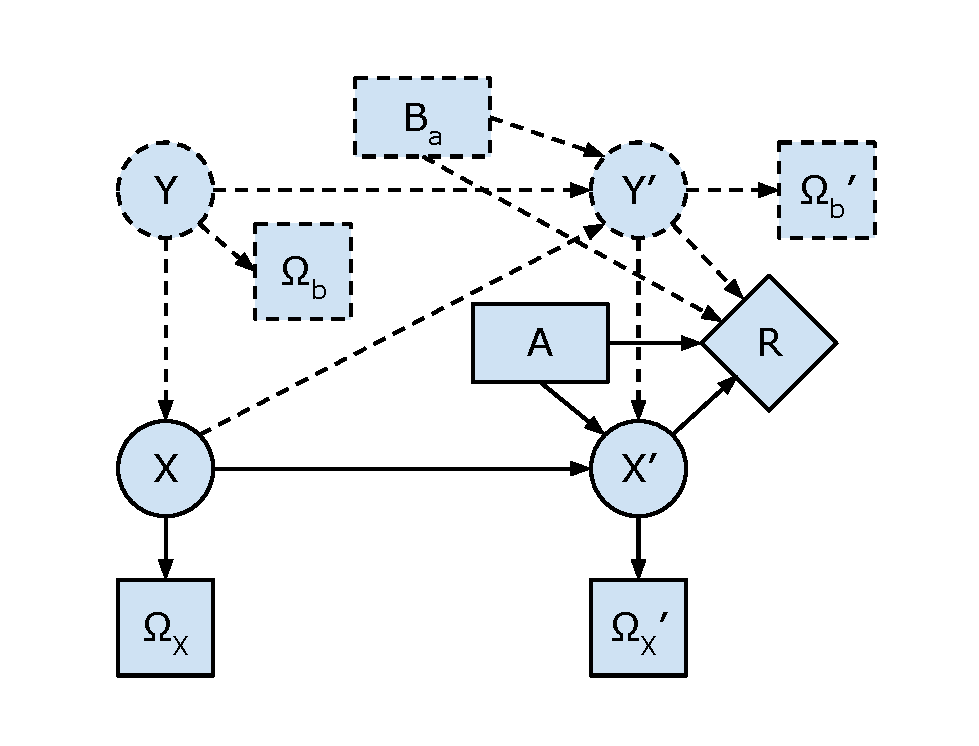
\includegraphics[trim = 15mm 10mm 15mm 10mm, clip, width=\linewidth]{fig/fig-pomdp.pdf}
\column{.5\textwidth}
\begin{itemize}
\item A timeslice of a POMDP process (solid lines)
\pause \item Variables: \{ $X$, $A$, $\mathbf{\Omega_{X}}$ \}
\pause \item $Pr : X \to \Delta(\mathbf{\Omega_{X}})$, $Pr : X \times A \to \Delta(\mathbf{X})$
\pause \item Reward Function: $R(A, X')$
\pause \item Augmented with affective \\ states (dotted lines)
\end{itemize}
\end{columns}
\end{frame}

%------------------------------------------------
\subsection{The BayesACT Framework}
\begin{frame}
\frametitle{Concepts - BayesACT}
\begin{itemize}
\item A Bayesian version of the ACT theory
\item Combines the ACT with POMDP model so that can learn an interactant's identity
\end{itemize}
%insert figure & explain the bayesact framework
\pause
\begin{columns}[c]
\column{.5\textwidth}
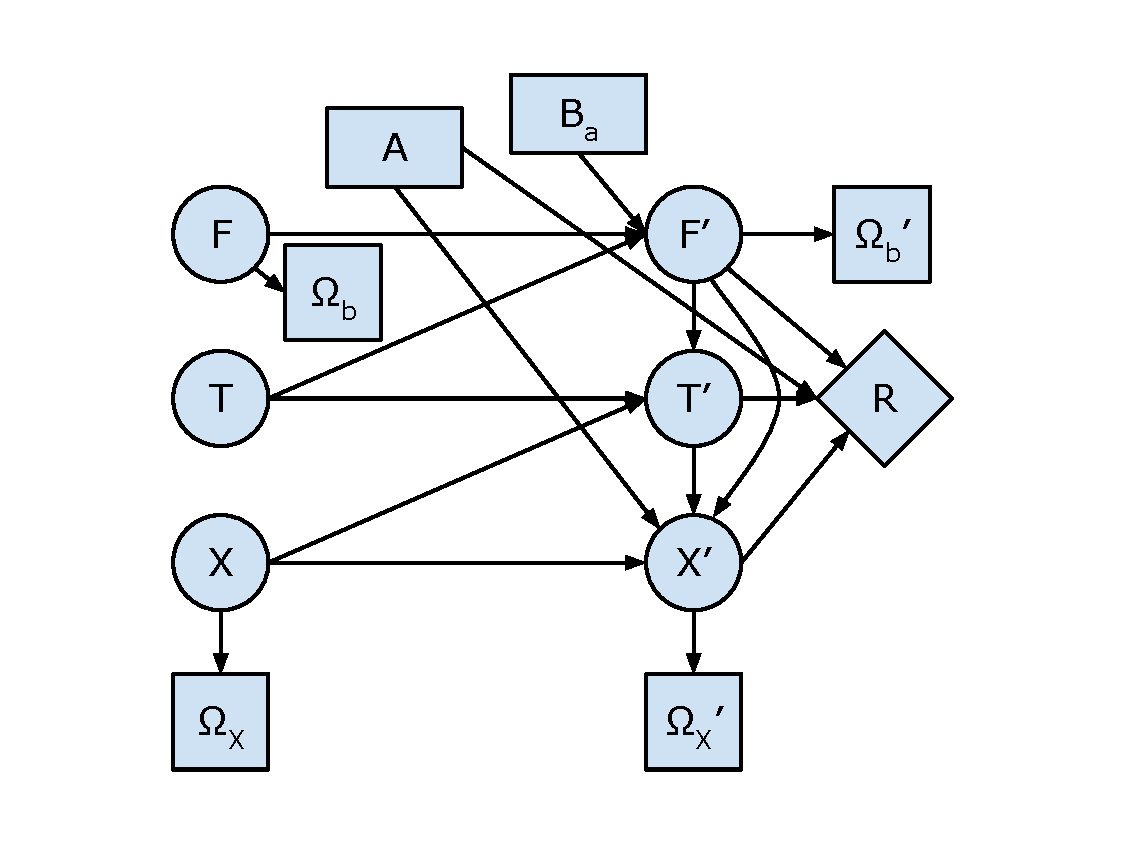
\includegraphics[trim = 20mm 10mm 20mm 10mm, clip, width=\linewidth]{fig/fig-bayesact.pdf}
\column{.5\textwidth}
\begin{itemize}
\pause \item States $S = \{F, T, X\}$, where $F = \{F_{ij}\}, T = \{T_{ij}\}, i \in \{a, b, c\}, j \in \{e, p, a\}$
\pause \item Observations $\Omega = \{\Omega_{X}, \Omega_{b}\}$
\pause \item Actions $\{A, B_{a}\}$
\pause \item By updating $F$, the probability distribution of the client's identity $F_{c}$ is learned
\pause \item Calculate $\{A, B_{a}\}$ basing on $\{F, T, X\}$
\end{itemize}
\end{columns}
\end{frame}

\begin{frame}
\frametitle{Concepts - BayesACT cont.}
Updates $F$ and Calculates $\{A, B_{a}\}$ basing on $\{F, T, X\}$
\begin{itemize}
% ---- formula computing deflection ----
\pause \item The deflection $\phi(F, T)$ between $F$ and $T$: 
\begin{equation}\label{eq:eq_deflection}
\phi(f,t) \propto e^{-(f'-t')\Sigma^{-1}(f-t)}
\end{equation}
% ---- formula computing probability of $f'$ ----
\pause \item The probability of a post-action fundamental sentiment $f'$:
\begin{equation}\label{eq:eq_pr_f}
Pr(f'|f,t,x,b_{a},\phi) \propto e^{-\phi(f',t')-\xi(f',f,b_{a},x)} 
\end{equation}
where $t'$ can be computed from $\{f', t, x\}$ by empirically derived prediction equations of ACT.
% ---- how the application progresses (i.e. how planstep changes in our case) ----
\pause \item $Pr(x'|x,f',t',a)$: how the application progresses
% ---- observation functions ----
\pause \item $Pr(\omega_{b}|f)$ and $Pr(\omega_{x}|x)$: observation functions for the client behaviour sentiment and system state 
\end{itemize}
\end{frame}

%-----------------------------------------------------------------
\section{Solution: System Design and Implementation}
%------------------------------------------------
\begin{frame}
\frametitle{Solution - Overview}
\begin{block}{Goal}
\small{
Design an \textit{extensible} system that assists \textit{people with dementia} during a hand-washing process by \textit{assessing their states} and \textit{provide instructions accordingly}.
}
\end{block}
%insert figure describing the functionality of each component of the system
%state how each component is related to our objective
\pause 
\begin{figure}
\centering
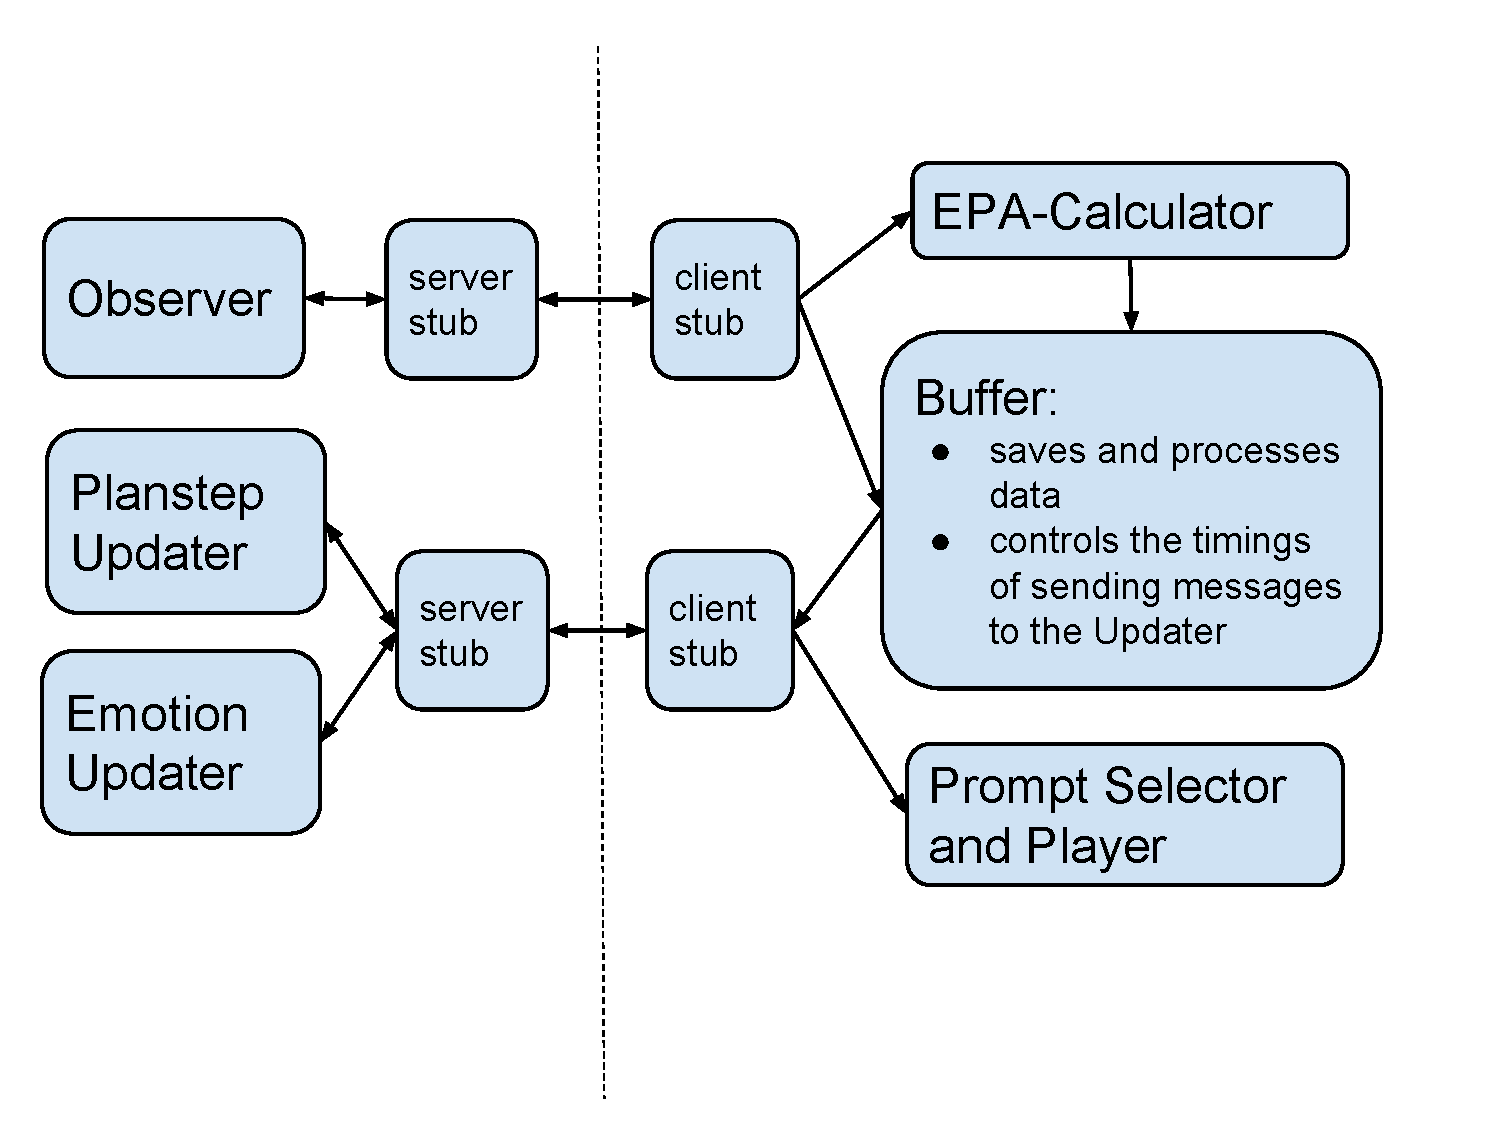
\includegraphics[trim = 5mm 15mm 5mm 20mm, clip, width=.8\linewidth]{fig/fig-system-overview.pdf}
\end{figure}
%state the server-client model is used & a "buffer" component is involved
%we focus on explaining how the servers is designed in "components" and then how they coordinate later
\end{frame}

%------------------------------------------------
\subsection{Components}

\begin{frame}
\frametitle{Solution - the Planstep and Emotion Updater}
%insert figure: designing & implementing the two updaters as a single reasoning engine
Design the Planstep and Emotion Updaters basing on the BayesAct code
\begin{figure}[htp]
\centering
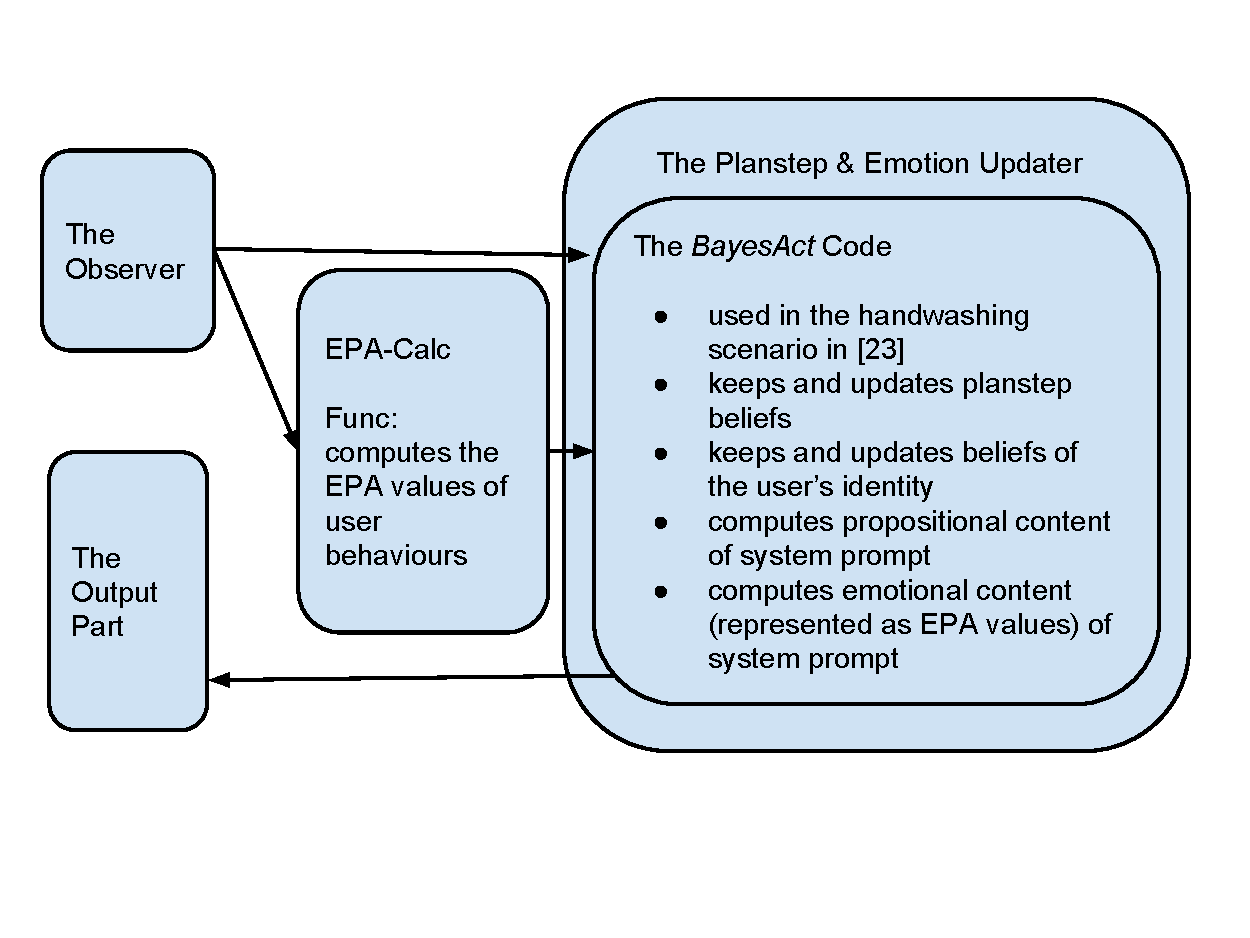
\includegraphics[trim = 4mm 30mm 5mm 15mm, clip, width=0.9\linewidth]{fig/fig-updater.pdf}
\label{fig:updater}
\end{figure}
\end{frame}

\begin{frame}
\frametitle{Solution - the Planstep and Emotion Updater cont.}
%planstep definitions: the 8 ps & 5 behaviours monitored
A planstep update diagram
\begin{figure}[htp]
\centering
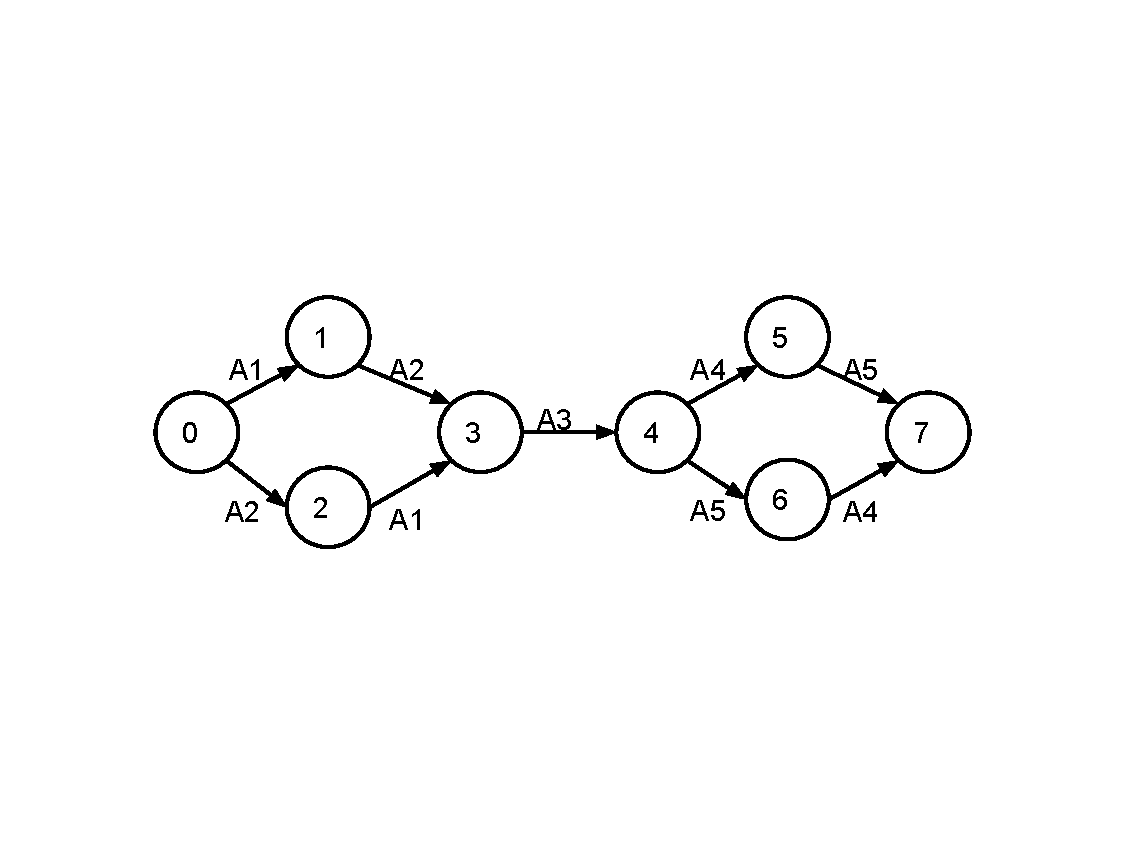
\includegraphics[trim = 20mm 50mm 20mm 50mm, clip, width=0.8\textwidth]{fig/fig-planstep.pdf}
\label{fig:planstep}
\end{figure}
\begin{itemize}
\pause \item Eight plansteps: (0) ``off/dirty/dry'', (1) ``on/dirty/dry'', (2) ``off/soapy/dry'', (3) ``on/soapy/dry'', (4) ``on/clean/wet'', (5) ``off/clean/wet'', (6) ``on/clean/dry'', (7) ``off/clean/dry''
\pause \item Five behaviours: A1 to A5 are ``turn on water'', ``put on soap'', ``rinse hands'', ``turn off water'', and ``use towel'', respectively.
\end{itemize}
\end{frame}

\begin{frame}
\frametitle{Solution - the Planstep and Emotion Updater cont.}
%insert figure: the model & how emotional states are updated (explaining how the bayesact framework works in a specific app scenario)
%note: there's a noise parameter describing the confidence of a certain result
Use the BayesACT framework in the handwashing scenario
\begin{itemize}
\item Recall: BayesACT includes states $S = \{X, F, T\}$, observations $\Omega = \{\Omega_{x}, \Omega_{b}\}$, and agent actions $\{A, B_{a}\}$
\pause \item In our hand-washing system, $X = \{X_{turn}, X_{ps}, X_{aw}, X_{bahav}\}$
\pause \item $\Omega_{x}$ gives evidence to the system about $X$
\pause \item $\Omega_{b}$ gives evidence to the system about $f_b$. The observation function $Pr(\Omega_b|f_b)$ allows one to specify the ``confidence'' or ``reliability'' of the different components of $\Omega_b$ by $\gamma$, which is the variance of a normal (Gaussian) distribution.
\pause \item Compute $X_{ps}'$ based on observation $\Omega_{x}$ and $\{X_{ps}, X_{behav}, X_{aw}, F, T\}$
\pause \item $A$ denotes the propositional content of a system message; $B_{a}$ denotes how the message should be expressed
\end{itemize}
\end{frame}

\begin{frame}
\frametitle{Solution - the Planstep and Emotion Updater cont.}
%insert figure: the model & how emotional states are updated (explaining how the bayesact framework works in a specific app scenario)
%note: there's a noise parameter describing the confidence of a certain result
Use the BayesACT framework in the handwashing scenario
\begin{itemize}
\item Recall: BayesACT includes states $S = \{X, F, T\}$, observations $\Omega = \{\Omega_{x}, \Omega_{b}\}$, and agent actions $\{A, B_{a}\}$
\pause \item In our hand-washing system, $X = \{X_{turn}, X_{ps}, X_{aw}, X_{bahav}\}$
\pause \item $\Omega_{x}$ gives evidence to the system about $X$
\pause \item $\Omega_{b}$ gives evidence to the system about $f_b$. The observation function $Pr(\Omega_b|f_b)$ allows one to specify the ``confidence'' or ``reliability'' of the different components of $\Omega_b$ by $\gamma$, which is the variance of a normal (Gaussian) distribution.
\pause \item Compute $X_{ps}'$ based on observation $\Omega_{x}$ and $\{X_{ps}, X_{behav}, X_{aw}, F, T\}$
\pause \item $A$ denotes the propositional content of a system message; $B_{a}$ denotes how the message should be expressed
\end{itemize}
\end{frame}

\begin{frame}
\frametitle{Solution - the EPA-Calculator}
\begin{itemize}
\item Essentially an ``Affect Recognition'' problem
\item Learns/ Calculates affective interpretations from user behaviours
%feature selection (other feature-selection approaches are not feasible in current situation)
\pause \item Feature Selection
\begin{itemize}
\item analysis on facial expressions and speeches
\item application scenario and user-group constraints
\end{itemize}
%describe the threshold-based method (i.e. piecewise linear interpolation)
\pause \item Calculate $P,A$ using piecewise linear interpolation method
\begin{itemize}
\item The average distance between the user's two hands in a set of $n$ neighbouring frames is scaled to $P$
\item The average distance the user's hands move between $n$ neighbouring frames is scaled to $A$
\end{itemize}
\pause \item Temporally smoothing in the Buffer
\begin{equation}
X=\sum_{k=i}^{j}(\dfrac{alpha}{alpha+1})^{j-k}*\dfrac{1}{alpha+1}*X[k]
\end{equation}
where $alpha \geq 0$, $X=P$ or $X=A$.
\end{itemize}
\end{frame}


\begin{frame}
\frametitle{Solution - the Observer}
\begin{itemize}
%state how the original hand-tracker works
\item Step 1: Get the locations of the user's hands
\begin{itemize}
\item utilize Czarnuch and Mihailidis's body tracker \cite{czarnuch2014}
\item the tracker obtains body parts locations from the depth information of images taken from an overhead perspective
\item the tracker was trained using partially labeled, unbalanced data, and is configurable and re-trainable\\
\pause
\begin{figure}[htb]
\centering
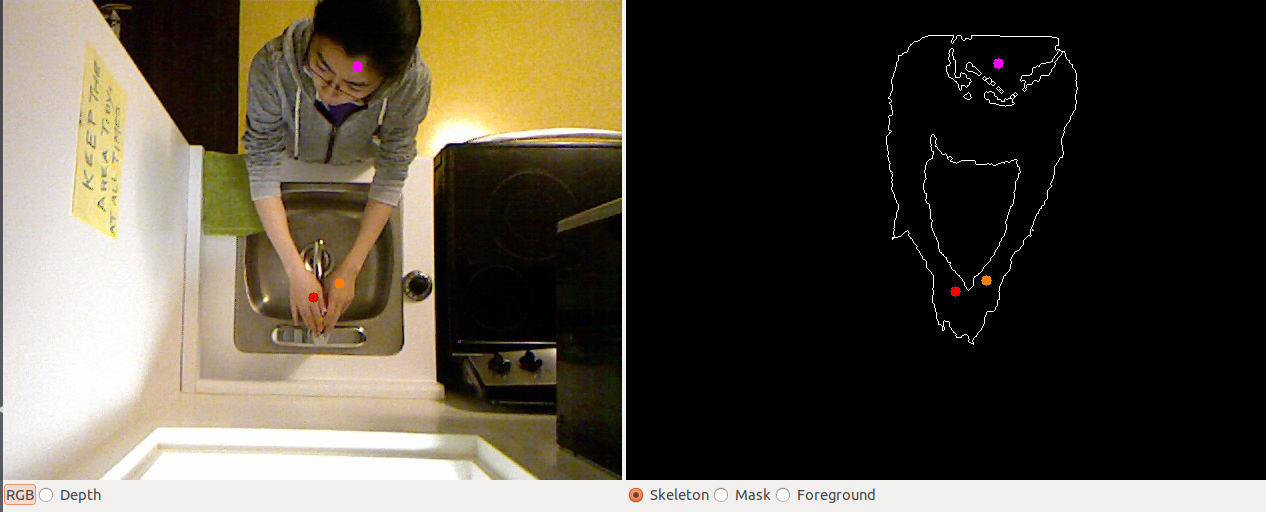
\includegraphics[width=0.9\linewidth]{fig/handtracker-performance.png}
\end{figure}
\end{itemize}
\end{itemize}
\end{frame}

\begin{frame}
\frametitle{Solution - the Observer cont.}
\begin{itemize}
\item Step 1: Get the locations of the user's hands
\begin{itemize}
\item utilize Czarnuch and Mihailidis's body tracker \cite{czarnuch2014}
\item the tracker obtains body parts locations from the depth information of images taken from an overhead perspective
\item the tracker was trained using partially labeled, unbalanced data, and is configurable and re-trainable
\end{itemize}
\item Step 2: Map locations to user behaviours
\begin{itemize}
\item compare hands locations with object positions
\item objects: the left-tap, the right-tap, the soap, the water-flow, the towel
\item observation noise handled by the observation function in the Reasoning Engine
\end{itemize}
%state the server-client model is used
\pause \item Serves as an Observer server
\begin{itemize}
\item with the help of the Buffer
\end{itemize}
\end{itemize}
\end{frame}

\begin{frame}
\frametitle{Solution - the Output Part}
\begin{itemize}
%describe the survey - insert figure: examples of the prompts
\item The prompt dataset: the audio-visual prompts generated and evaluated in Malhotra's study \cite{malhotra2014}
\begin{itemize}
\item created 30 video clips using the USC Virtual Human Toolkit
\item EPA values of videos evaluated by human raters
\item the participants' answers are consistent with each other
\end{itemize}
%figure: Screenshots of two video prompts stating same propositional messages
\begin{figure}[htb]
\centering
\begin{subfigure}[b]{.4\textwidth}
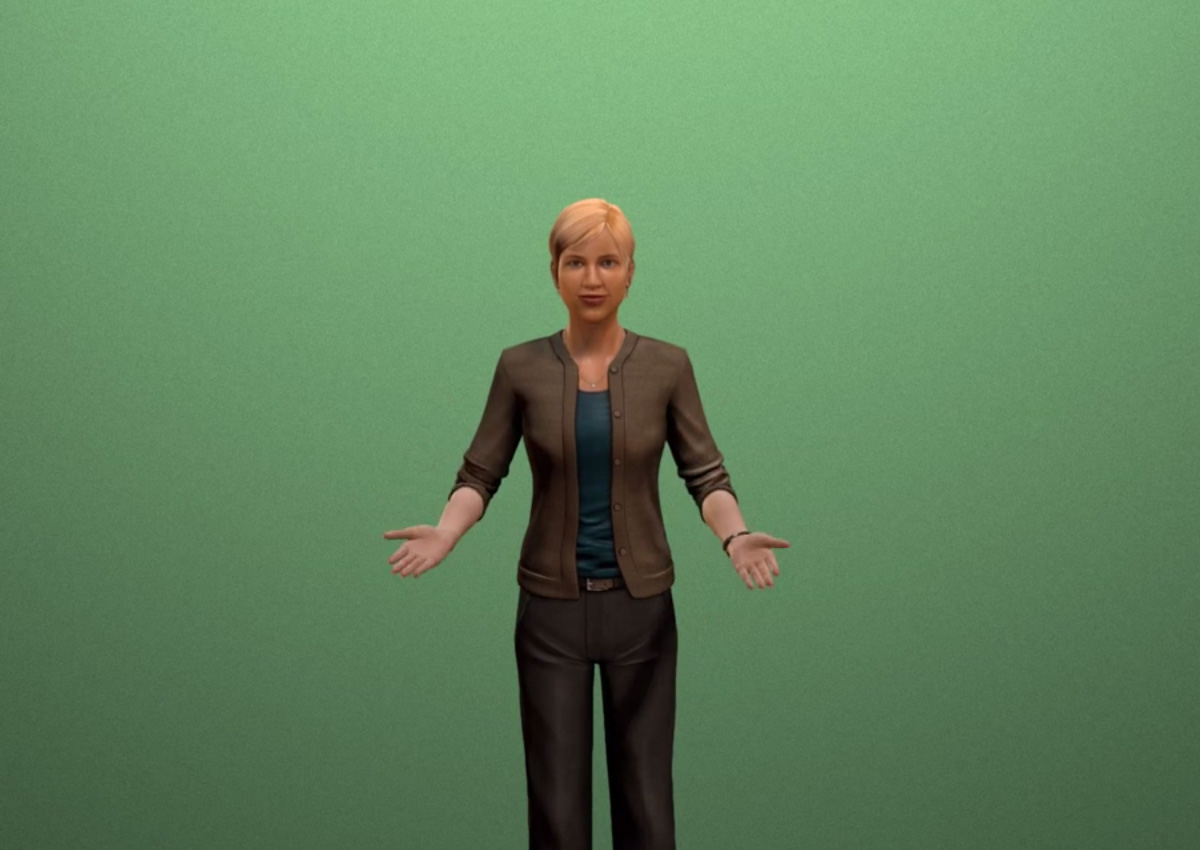
\includegraphics[width=\textwidth]{fig/prompt1.jpg}
\end{subfigure}
\begin{subfigure}[b]{.4\textwidth}
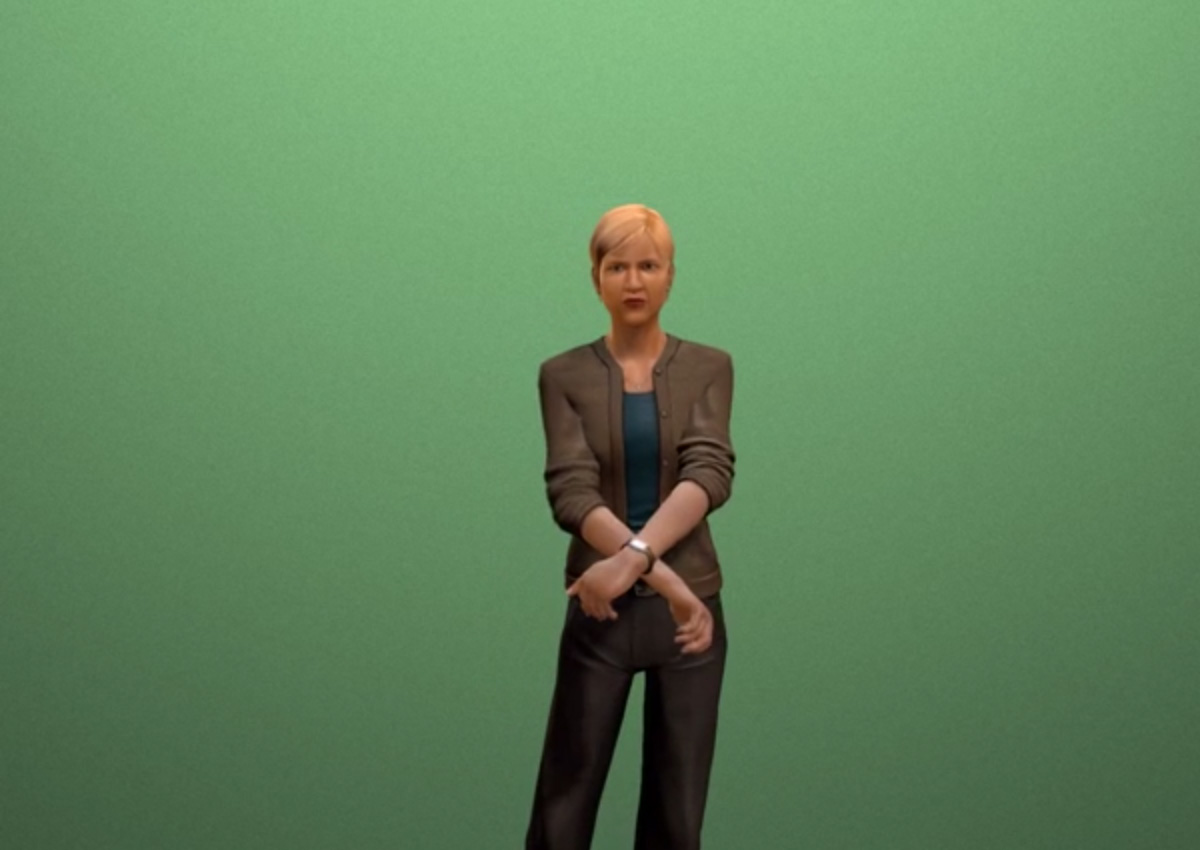
\includegraphics[width=\textwidth]{fig/prompt2.jpg}
\end{subfigure}
\end{figure}
%describe how to select (include formula defining the distance of prompts)
\pause
\item A proper prompt is selected as the final prompt if it:
\begin{itemize}
\item has the same propositional labels as the desired prompt
\item has the closest emotional (EPA) values as the desired prompt
\end{itemize}
\end{itemize}
\end{frame}

%------------------------------------------------
\subsection{Coordination between components}

\begin{frame}
\frametitle{Solution - Coordination between components}
\begin{itemize}
\item The system is designed with independent components.
\begin{figure}
\centering
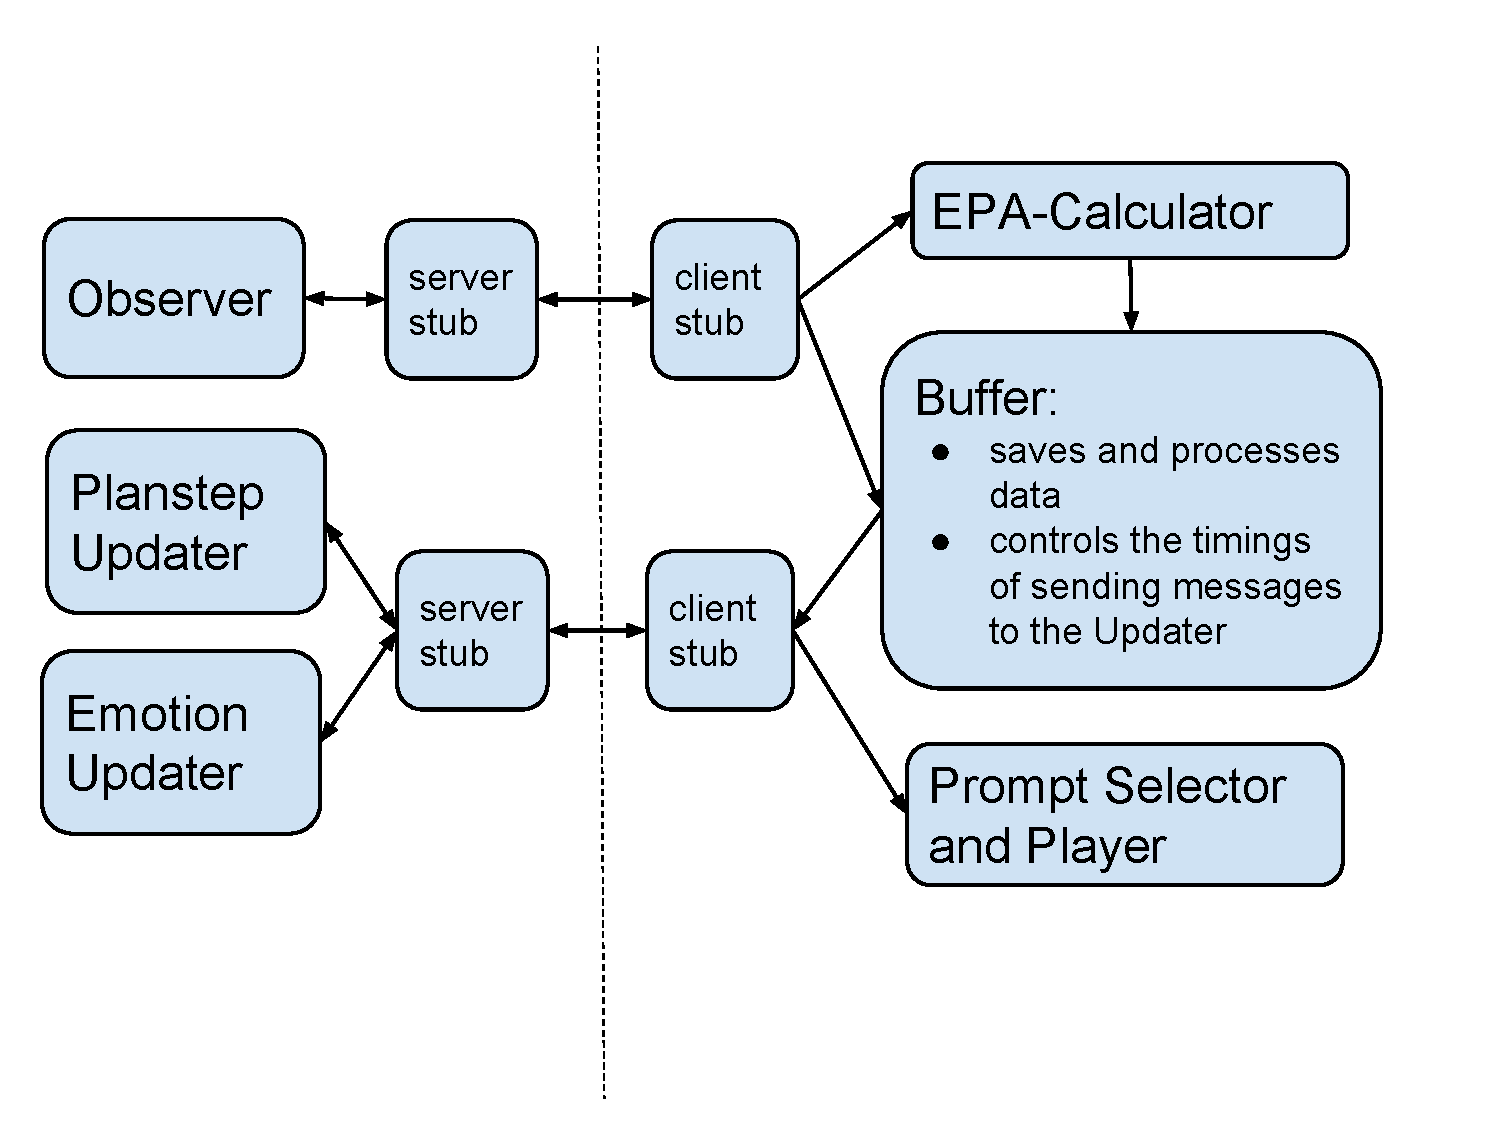
\includegraphics[trim = 5mm 35mm 5mm 20mm, clip, width=.8\linewidth]{fig/fig-system-overview.pdf}
\end{figure}
%state the server-client model is used & a "buffer" component is involved
\item How to coordinate between the components?
\begin{itemize}
\item timings of sending request and response messages?
\end{itemize}
\end{itemize}
\end{frame}

\begin{frame}
\frametitle{Solution - The Buffer}
\begin{itemize}
\item Between the Observer, the EPA-Calc, and the Reasoning Engine
\item Controls timings of sending messages
\begin{figure}
\centering
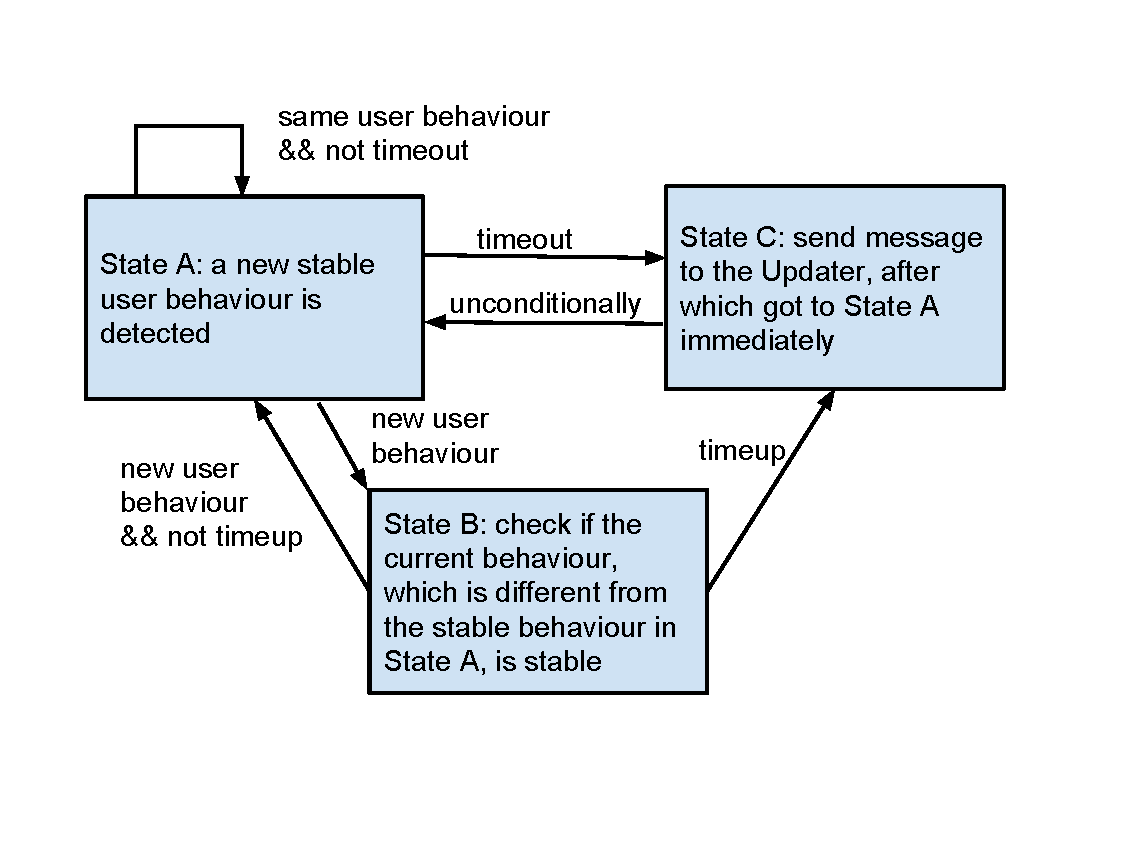
\includegraphics[trim = 10mm 25mm 16mm 15mm, clip, width=0.75\linewidth]{fig/fig-state-trans.pdf}
\end{figure}
\item Smoothes EPA values calucated by the Calculator
\end{itemize}
\end{frame}

%-----------------------------------------------------------------
\section{Experimental Results}
%-----------------------------------------------------------
\begin{frame}
\frametitle{Experiments - Variables and Parameters}
%locations of "certain objects": related to the 5 behaviours (give a screenshot of the physical settings; or mention would give)
\end{frame}

\begin{frame}
\frametitle{Experiments - Variables and Parameters cont.}
%table defining all the parameters - explain the meanings of all the parameters
\end{frame}

\begin{frame}
\frametitle{Experiments - Test \#1}
%table 1 + video 1: what happened in run 1
%explanation focus on planstep responses
%mention emotional responses in general
\end{frame}

\begin{frame}
\frametitle{Experiments - Test \#1 cont.}
%(if needed) table 1 + video 1: what happened in run 1
\end{frame}

\begin{frame}
\frametitle{Experiments - Test \#2}
%video 2 + table 2: what happened in run 2
%explanation focus on planstep responses
%mention emotional responses in general
\end{frame}

\begin{frame}
\frametitle{Experiments - Test \#2 cont.}
%(if needed) table 2: what happened in run 2
\end{frame}

\begin{frame}
\frametitle{Experiments - Conclusion}
%planstep updater - they can update accordingly
%emotion updater - insert table & state the correlations found between EPA values
%mention that more experiments were run & result is in the appendix 
\end{frame}

%-----------------------------------------------------------------
\section{Discussion}
%-----------------------------------------------------------

\subsection{Contribution}
\begin{frame}
\frametitle{Discussion - Contribution}
%review the four objectives
%state contribution of this paper
\end{frame}

\subsection{Future Work}
\begin{frame}
\frametitle{Discussion - Future Work}

\end{frame}

%---------------------------------------------------------------
% Ending pages
%---------------------------------------------------------------
\begin{frame}
\frametitle{References}
[1] The bayesact paper
\newline [2] The tracker paper.
\newline [3] The survey paper.
\end{frame}
%------------------------------------------------
\begin{frame}
\frametitle{Acknowledgement}
Jesse Hoey
\newline James Tung and Peter van Beek
\newline Xiao Yang, Chengbo Li and Enxun Wei
\end{frame}
%------------------------------------------------
\begin{frame}
\frametitle{The end}
\Huge{\centerline{Thank you!}}   
\fontsize{5mm}{4mm}
\begin{itemize}
\item Questions?
\item Comments?
\end{itemize}
\end{frame}
%----------------------------------------------------------------------------------------

%---------------------------------------------------------------
% Additional pages
% put pages in assistance to answering questions here
%---------------------------------------------------------------

%pseudo-code page(1): how planstep is updated according to behavioural obs, awareness, & deflection
\begin{frame}
\frametitle{Update $X_{ps}'$ based on $\Omega_{x}$ and $\{X_{ps}, X_{behav}, X_{aw}, F, T\}$}
\begin{itemize}
\item $SampleXVar()$ and $evalSampleXVar()$
\item Pseudocode of $SampleXVar()$
\end{itemize}
\end{frame}

%pseudo-code page(2): how planstep is updated according to behavioural obs, awareness, & deflection
\begin{frame}
\frametitle{Update $X_{ps}'$ based on $\Omega_{x}$ and $\{X_{ps}, X_{behav}, X_{aw}, F, T\}$ cont.}
%----------------- second item -----------------
\algsetup{linenosize=\scriptsize}
\begin{algorithm}[H]
\scriptsize
\begin{multicols}{2}
\begin{algorithmic}[1]
\IF {Deflection(F, T) is high} \STATE {
  threshold = high
} \ELSE \STATE {
  threshold = low
} \ENDIF
\IF {aw high} {
  \IF {prompted} {
    \IF{$random\_prob() <$ threshold} \STATE {
       aw = low and not moving forward
    } \ELSIF {prompt wrong} \STATE {
       aw = low and not moving forward
    } \ELSIF {likely} \STATE {
       moving forward
    } \ELSIF {$random\_prob() <$ threshold} \STATE {
       aw = low and not moving forward
    } \ENDIF
  } \ELSE {
    \IF {$random\_prob() <$ threshold} \STATE {
      aw = low and not moving forward
    } \ELSE \STATE {
      aw stays high and moving forward
    } \ENDIF
  } \ENDIF
} \ELSE {
  \IF {prompted} {
    \IF {$random\_prob() >$ threshold \AND prompt correct} \STATE {
	move on and aw high
    } \ELSE \STATE {
        unlikely: aw high and not moving forward
    } \ENDIF
  } \ELSE \STATE {
      unlikely: aw high and moving forward
  } \ENDIF
} \ENDIF
\end{algorithmic}
% compile k
\end{multicols}
\end{algorithm}
\end{frame}

%pseudo-code page(3): how planstep is updated according to behavioural obs, awareness, & deflection
\begin{frame}
\frametitle{Update $X_{ps}'$ based on $\Omega_{x}$ and $\{X_{ps}, X_{behav}, X_{aw}, F, T\}$ cont.}
\begin{itemize}
\item $SampleXVar()$ and $evalSampleXVar()$
\item Pseudocode of $SampleXVar()$
\pause \item $Pr: X_{behav} \to \Delta(\Omega_{x})$ used in $evalSampleXVar()$
\end{itemize}
\end{frame}

\end{document} 
